\begin{frame}{Before We Start!!!}
    \setbeamercovered{transparent}
    \begin{itemize}
        \item Before we dive into the discussions of Flip-flops, let's go for a quick introduction of it!
        \pause
        \item And for that, we will need to know about one important concept first! 
    \end{itemize}
\end{frame}

\begin{frame}{Sequential Circuits}
    \begin{itemize}
        \item We know, pretty much in everywhere, output depends on input.
        \pause
        \item Putting it more formally in case of circuits... \textcolor{blue}{present output depends on present input.}
        \pause
        \item \textbf{But output of sequential circuits depend on past output too!!!}
    \end{itemize}
\end{frame}

\begin{frame}{Sequential Circuits (contd.)}
    \begin{itemize}
        \item That brings an important point: we need to \alert{store} the past output somewhere.
        \pause
        \item For that, we need storage devices. 
        \pause
        \item And here is where \textbf{Flip-flop} comes in play.
        \pause
        \item This whole thing is also known as \textcolor{blue}{storing the state of our circuit.}
    \end{itemize}
\end{frame}

\begin{frame}{Two Important Questions}
\begin{enumerate}
    \item What does Flip-flop do?
    \begin{itemize}
        \item It stores and updates the state of our circuit
    \end{itemize}
    \pause
     \item How does it know when to update the state?
    \begin{itemize}
        \item It updates upon receiving a signal, whom we refer to as \textcolor{blue}{clock}
        \break
        \begin{figure}
            \centering
            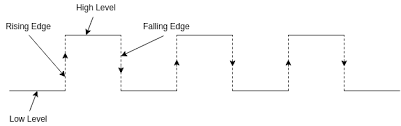
\includegraphics[width=0.8\textwidth]{download.png}
            \label{fig:my_label}
        \end{figure}
    \end{itemize}
\end{enumerate}
\end{frame}